%% 
%% Copyright 2007-2020 Elsevier Ltd
%% 
%% Este arquivo é uma adaptação de arquivo do pacote 'Elsarticle', que está disponível respeitando-se os termos da licença 'LaTeX Project Public License', na versão 1.2 ou posterior. 
%%-------------------------------------------------------------


\documentclass[12pt]{elsarticle}

%% para incluir figuras, graphicx.sty foi adicionado ao arquivo
%% elsarticle.cls. Se você prefere comandos mais antigos
%% por favor, adicione o pacote \usepackage{epsfig}

%% O pacote amssymb contém cários símbolos matemáticos úteis
\usepackage{amssymb}

%% O pacote babel coloca acentuação e hifenização de acordo com o português (Brasil)
\usepackage[brazil]{babel}

%%usando padrão utf8 para codificação
\usepackage[utf8]{inputenc}

%% O pacote amsthm contém a definição de alguns ambientes matemáticos
\usepackage{amsthm}

%configuração das margens
\usepackage[left=2.5cm, right=2.5cm, top=4cm, bottom=3cm, footskip=0.5cm]{geometry}

%supressão dos números de página
\pagenumbering{gobble}

\journal{ }

\begin{document}

\begin{frontmatter}

\title{Quantum Oracles - Como transformar problemas clássicos em quânticos}

\date{ \today }

\author[1,*]{Alexandre Silva}
\author[1]{Luis Hilário Tobler Garcia}
\author[2]{Maúricio Duarte}

\address[1]{UNIVEM - Centro Universitário Eurípides de Marília, Avenida Hygino Muzzi Filho, Marília-SP}
\address[2]{Fatec Garça – Deputado Julio Julinho Marcondes de Moura, Av. Pres. Vargas, 2331 - José Ribeiro, Garça-SP}

\address[*]{Autor para correspondência: alexandresilvaunivem@gmail.com}


%Resumo 
\begin{abstract}
%% Texto do resumo
\begin{resumop}
A partir do uso de quantum Oracles e outros fatores quânticos, como a superposição, foram feitos \emph{5 mini-projetos}. O objetivo desses projetos foi tentar responder se é possível transformar certos problemas em quânticos e se realmente tal transformação vale a pena. Após os testes foi possível ver que, há casos em que a versão quântica apresenta um aproveitamento igual ou um pouco superior, contudo ainda é necessário o uso de computadores clássicos para conseguir melhores resultados.
\end{resumop}

\begin{resumoi}
Using quantum Oracles and other quantum factors, such as superposition, \emph{5 mini-projects} were carried out. The aim of these projects was to try to answer whether it is possible to transform certain problems into quantum ones and whether such a transformation is really worthwhile. After the tests, it was possible to see that there are cases in which the quantum version shows equal or slightly better performance, but it is still necessary to use classical computers to achieve better results.
\end{resumoi}
\end{abstract}

\begin{keyword}
%% palavras-chaves devem ser colocadas aqui, no seguinte formato: palavra1 \sep palavra2 \sep palavra3
quantum oracles \sep quantum algorithms \sep quantum computing
\end{keyword}

\end{frontmatter}

%% testo princicpal
\section{Mini-projetos}
\label{sec:impl}

%% Para citações use: 
%%       \citet{<label>} ==> Jones et al. [21]
%%       \citep{<label>} ==> [21]
%%
Durante a pesquisa, foram criados 5 mini-projetos: Explorador de Arquivos, conversão de milhas para quilômetros, Torres de Hanoi, Buckshot Roulette e QRAM. Todos utilizando dos Quantum Oracles, alguns algoritmos, explorando efeitos quânticos, e algumas técnicas, tanto clássicas como quânticas, para cada projeto específico. Contudo, para essa publicação será focado apenas no Buckshot Roulette, projeto do qual obteve melhores resultados e mais técnicas puderam ser aproveitadas.

\section{Buckshot Roulette}
\label{sec:bck}
Buckshot Roulette é um jogo de computador que se tornou viral no começo de 2024, por sua mecânica inspirada na infame roleta russa. O jogo despertou minha curiosidade para conseguir encontrar a melhor estratégia para o jogador vencer a maior parte do tempo. Para isso, foi implementada uma versão quântica do jogo, simulando a primeira rodada.

Para isso, foi criado um circuito quântico, utilizando o Qiskit, simulando cara interação entre player e adversário. Além disso, para inserir a estratégia de cada um no circuito, foram criados dois Oracles e dentro do referente ao player foram adicionados parâmetros, usados para facilitar manipulação os valores de rotação na Bloch Sphere conforme necessário.

Com isso, o circuito foi simulado $1000$ vezes para cada combinação de estratégia, com o objetivo de maximar os ganhos do jogador. A cada iteração, um valor diferente era adicionado para $\theta$ e $\phi$, num range de $[{\pi\over{4}}, \pi[$ e $[{\pi\over{4}}, 2\pi[$ respectivamente. Ao final da simulação, os melhores valores foram: $\theta\approx 3.0853981633974477, \phi\approx3.7853981633974474$ radianos.


\begin{figure}[h]
	\centering
	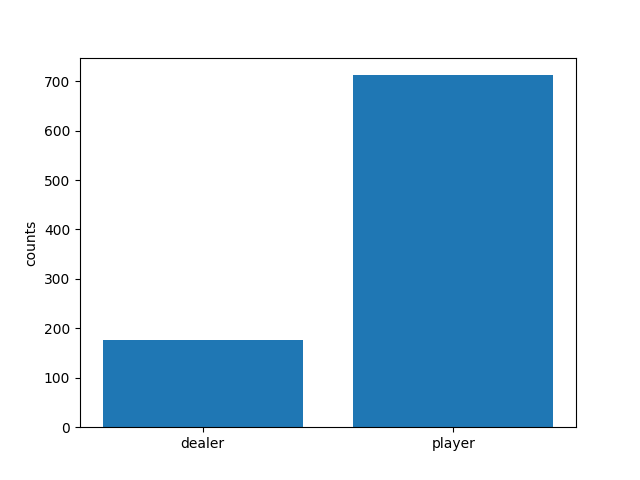
\includegraphics[width=0.5\textwidth]{final_buckshot_roulette_quantum_optimal_strategy}
	\caption{Versão quântica - resultados}
	\label{fig:quantum-version}
\end{figure}

Ao comparar os resultados com o da versão clássica, foi possível ver que os resultados são muito próximos, sendo o player vencedor em $\approx 70\%$ das vezes. Com isso, foi demonstrado que é possível simular tal jogo usando computação quântica, e também que tal versão pode se sobressair ao seu relativo de computação clássica, uma vez que pode-se explorar mais estrategias, devido a ampla gama de rotações na Bloch Sphere.

%% Se você tem um arquivo bib e quer que o  bibtex gere os 
%% bibitems, por favor, use:
%%

\nocite{alexandre_2024_dpbmscientificinitiation1quantumoracles}
\nocite{klubnika_2023_buckshot}

\bibliographystyle{elsarticle-num-names} 
\bibliography{references} %no lugar de cas-refs coloque o nome do seu arquivo .bib

%% senão use o seguinte código para adicionar as entradas dos bibitems diretamente no arquivo TeX.

% \begin{thebibliography}{00}

% %% \bibitem[Autor(ano)]{label}
% %% Texto do item bibliográfico

% \bibitem[ ()]{}

% \end{thebibliography}
\end{document}

\endinput
%%
%% Fim o arquivo main.tex'.
